\documentclass{beamer}
\usepackage{etex} % to avoid errors http://tex.stackexchange.com/questions/7896/no-room-for-a-new-dimen-when-including-tikz
\usepackage{ulem}
\usepackage{listings}
\usepackage{slashbox}
\usepackage{tikz}
\usepackage[all]{xy}
\usepackage{booktabs}
\usepackage{amsmath,amssymb}
\usepackage{hyperref}
\usepackage{graphicx}

\DeclareMathOperator*{\argmin}{arg\,min}
\DeclareMathOperator*{\argmax}{arg\,max}
\DeclareMathOperator*{\maximize}{maximize}
\DeclareMathOperator*{\minimize}{minimize}
\newcommand{\sign}{\operatorname{sign}}
\newcommand{\RR}{\mathbb R}
\newcommand{\NN}{\mathbb N}

% Set transparency of non-highlighted sections in the table of
% contents slide.
\setbeamertemplate{section in toc shaded}[default][100]
\AtBeginSection[]
{
  \setbeamercolor{section in toc}{fg=red} 
  \setbeamercolor{section in toc shaded}{fg=black} 
  \begin{frame}
    \tableofcontents[currentsection]
  \end{frame}
}

\begin{document}

\title{Supervised, interactive genomic data analysis}
\author{
Toby Dylan Hocking
}

\date{Barbados workshop, 5--9 January 2015}

\maketitle

\section{Some problems with unsupervised
  DNA copy number analysis}

\begin{frame}
  \frametitle{DNA copy number analysis}

  Figure source: Alberts \textit{et al.} 2002. Molecular Biology of the Cell.
\vskip 0.1in
  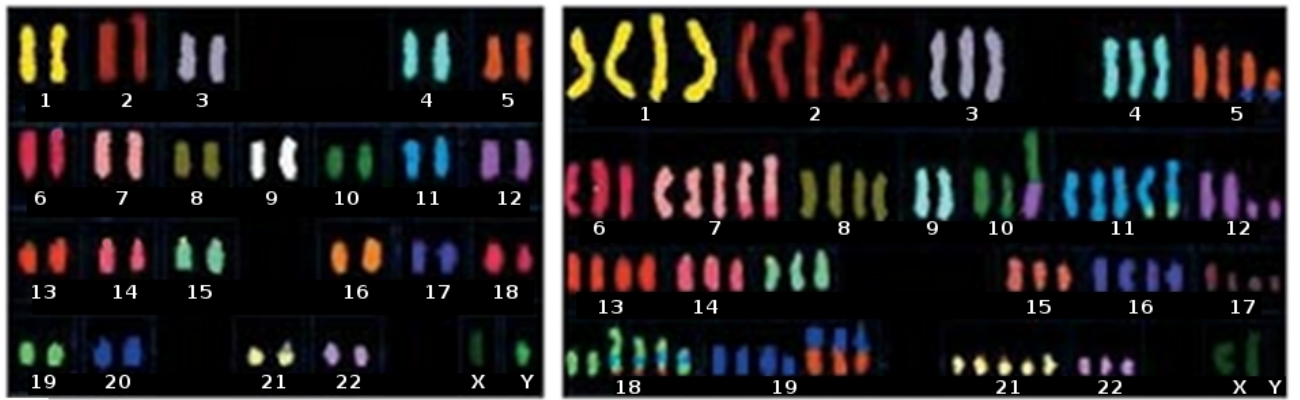
\includegraphics[width=\textwidth]{Karyo-both}
\vskip 0.1in
  \begin{minipage}{0.4\linewidth}
    Normal cell with 2 copies of each autosome.
  \end{minipage}
\hskip 0.1\linewidth
  \begin{minipage}{0.4\linewidth}
Cancer cell with many copy number alterations.
  \end{minipage}

\end{frame}

\begin{frame}
  \frametitle{Unsupervised, non-interactive DNA copy number analysis}
  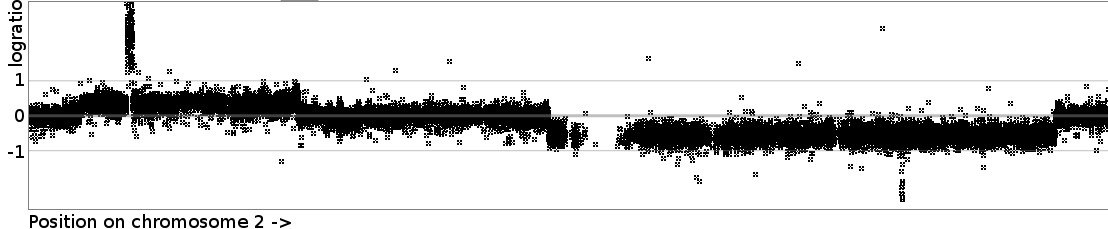
\includegraphics[width=\textwidth]{unlabeled-axes}

  Analyst sees a vector of $d$ noisy data points $\mathbf x\in\RR^d$.

  \vskip 0.1in

  \textbf{Question:}\\
  where are the true changes in copy
  number? (breakpoints)

\end{frame}

\begin{frame}
  \frametitle{Unsupervised, non-interactive DNA copy number analysis}

  \textbf{Unsupervised default model:} 
  fit a breakpoint model $f(\mathbf x, \lambda)$.\\
  ($\lambda$ is a model parameter, for example a p-value threshold or
  the number of breakpoints)

  \begin{displaymath}
  \xymatrix{
    \text{Data $\mathbf x$}
    \ar `[r] [dr] 
    & \text{ }
    \\
    % \text{Plot} \ar@{->}[d]
    & 
    \text{Model $f(\mathbf x, \lambda)$} 
    \\
    % \text{Labels $\mathbf y$}       \ar@{->}[d]
    \\
    \text{Parameter $\lambda$} 
    \ar `r[ruu] [ruu]
    & \text{ }
  }
  \end{displaymath}
  
  \textbf{Problem}: how do we know the model $f$ and parameter
  $\lambda$ are reasonable?

  \vskip 0.1in

  \textbf{Solution:} plot breakpoints $f(\mathbf x, \lambda)$ and
  interactively choose a reasonable parameter $\lambda$.
\end{frame}

\begin{frame}
  \frametitle{Unsupervised, interactive DNA copy number analysis}
  Analyst sees a vector of $d$ noisy data points $\mathbf x\in\RR^d$, \\
  and the model breakpoints $f(\mathbf x, \lambda)$.

  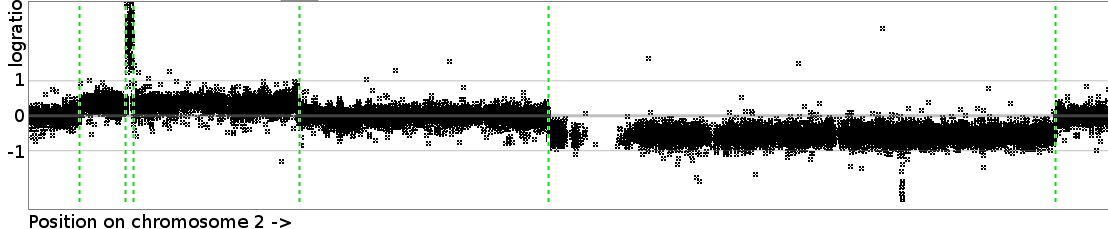
\includegraphics[width=\textwidth]{unlabeled-breakpoints-6}

  Parameter $\lambda$ = 6 breakpoints.
\end{frame}

\begin{frame}
  \frametitle{Unsupervised, interactive DNA copy number analysis}
  Analyst sees a vector of $d$ noisy data points $\mathbf x\in\RR^d$, \\
  and the model breakpoints $f(\mathbf x, \lambda)$.

  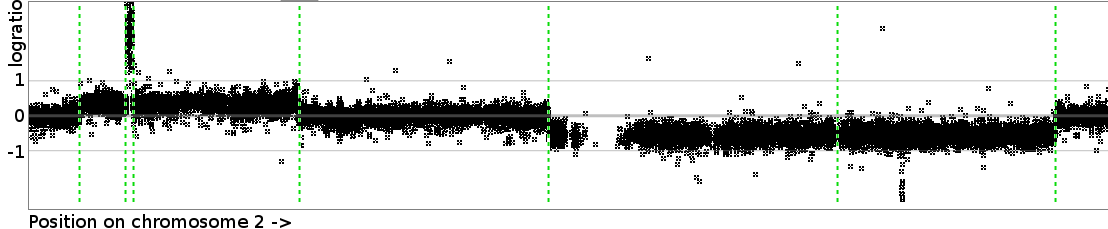
\includegraphics[width=\textwidth]{unlabeled-breakpoints-7}

  Parameter $\lambda$ = 7 breakpoints.
\end{frame}

\begin{frame}
  \frametitle{Unsupervised, interactive DNA copy number analysis}
  Analyst sees a vector of $d$ noisy data points $\mathbf x\in\RR^d$, \\
  and the model breakpoints $f(\mathbf x, \lambda)$.

  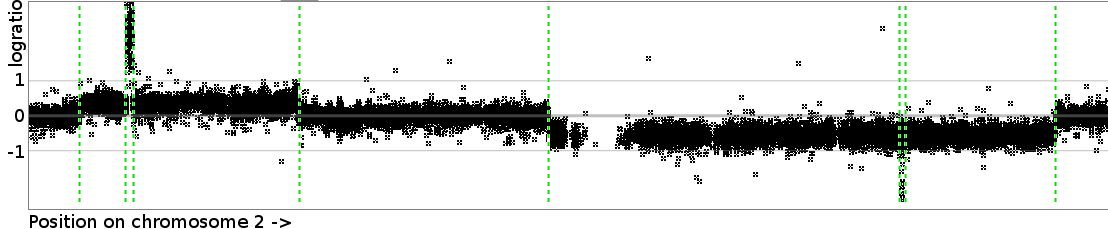
\includegraphics[width=\textwidth]{unlabeled-breakpoints-8}

  Parameter $\lambda$ = 8 breakpoints.
\end{frame}

\begin{frame}
  \frametitle{Unsupervised, interactive DNA copy number analysis}
  Analyst sees a vector of $d$ noisy data points $\mathbf x\in\RR^d$, \\
  and the model breakpoints $f(\mathbf x, \lambda)$.

  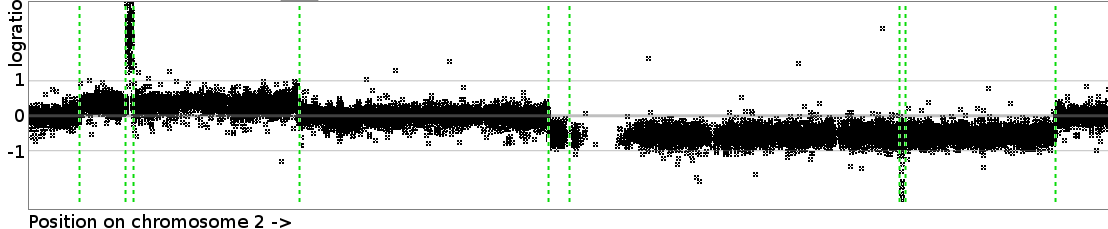
\includegraphics[width=\textwidth]{unlabeled-breakpoints-9}

  Parameter $\lambda$ = 9 breakpoints.
\end{frame}

\begin{frame}
  \frametitle{A brief history of unsupervised DNA copy number analysis}
  \begin{itemize}
  \item GLAD: adaptive weights smoothing (Hup\'e \textit{et al.}, 2004)
  \item DNAcopy: circular binary segmentation (Venkatraman and Olshen,
    2007)
  \item cghFLasso: fused lasso signal approximator with heuristics
    (Tibshirani and Wang, 2007)
  \item HaarSeg: wavelet smoothing (Ben-Yaacov and Eldar, 2008)
  \item GADA: sparse Bayesian learning (Pique-Regi \textit{et al.}, 2008)
  \item flsa: fused lasso signal approximator path algorithm (Hoefling 2009)
  \item cghseg: pruned dynamic programming (Rigaill 2010)
  \item PELT: pruned exact linear time (Killick \textit{et al.}, 2011)
  \end{itemize}
  Demo: \url{http://compbio.med.harvard.edu/CGHweb/}
\end{frame}

\begin{frame}
  \frametitle{Unsupervised, interactive DNA copy number analysis}
  
  Non-interactive unsupervised default model.
  
  \small

  \begin{displaymath}
  \xymatrix{
    \text{Data $\mathbf x$}
    \ar `[r] [dr] 
    %\ar `r[rr] [drr] 
    %\ar `r[rrr] [drrr] 
    %\ar [d]
    & \text{ }
    & \text{ }
    & \text{ }
    \\
    %\text{Plot} 
    %\ar [d]
    & 
    \text{Model $f(\mathbf x, \lambda_1)$} 
    %\ar [r]
    & 
    \textcolor{white}{\text{Plot}}
    %\ar[dd]
    &
    \color{white}{ \text{Model $f(\mathbf x, \lambda_2)$} }
    \\
    %\text{Labels $\mathbf y$}       
    %\ar [d]
    & 
    &
    \\
    \text{Parameter $\lambda_1$} 
    \ar `r[ruu] [ruu]
    %\ar [rr]
    & \text{ }
    & \color{white}{ \text{Parameter $\lambda_2$} }
    %\ar `r[ruu] [ruu] 
  }
  \end{displaymath}
\end{frame}

\begin{frame}
  \frametitle{Unsupervised, interactive DNA copy number analysis}

  Plot the default model.
  
  \small

  \begin{displaymath}
  \xymatrix{
    \text{Data $\mathbf x$}
    \ar `[r] [dr] 
    \ar `r[rr] [drr] 
    %\ar `r[rrr] [drrr] 
    %\ar [d]
    & \text{ }
    & \text{ }
    & \text{ }
    \\
    %\text{Plot} 
    %\ar [d]
    & 
    \text{Model $f(\mathbf x, \lambda_1)$} 
    \ar [r]
    & 
    \text{Plot}
    %\ar[dd]
    &
    \color{white}{ \text{Model $f(\mathbf x, \lambda_2)$} }
    \\
    %\text{Labels $\mathbf y$}       
    %\ar [d]
    & 
    &
    \\
    \text{Parameter $\lambda_1$} 
    \ar `r[ruu] [ruu]
    %\ar [rr]
    & \text{ }
    & \color{white}{ \text{Parameter $\lambda_2$} }
    %\ar `r[ruu] [ruu] 
  }
  \end{displaymath}
\end{frame}

\begin{frame}
  \frametitle{Unsupervised, interactive DNA copy number analysis}

  Increase/decrease parameter based on signal/noise in plot.
  
  \small

  \begin{displaymath}
  \xymatrix{
    \text{Data $\mathbf x$}
    \ar `[r] [dr] 
    \ar `r[rr] [drr] 
    %\ar `r[rrr] [drrr] 
    %\ar [d]
    & \text{ }
    & \text{ }
    & \text{ }
    \\
    %\text{Plot} 
    %\ar [d]
    & 
    \text{Model $f(\mathbf x, \lambda_1)$} 
    \ar [r]
    & 
    \text{Plot}
    \ar[dd]
    &
    \color{white}{ \text{Model $f(\mathbf x, \lambda_2)$} }
    \\
    %\text{Labels $\mathbf y$}       
    %\ar [d]
    & 
    &
    \\
    \text{Parameter $\lambda_1$} 
    \ar `r[ruu] [ruu]
    \ar [rr]
    & \text{ }
    & \text{Parameter $\lambda_2$}
    %\ar `r[ruu] [ruu] 
  }
  \end{displaymath}
\end{frame}

\begin{frame}
  \frametitle{Unsupervised, interactive DNA copy number analysis}

  Fit model using new parameter.
  
  \small

  \begin{displaymath}
  \xymatrix{
    \text{Data $\mathbf x$}
    \ar `[r] [dr] 
    \ar `r[rr] [drr] 
    \ar `r[rrr] [drrr] 
    %\ar [d]
    & \text{ }
    & \text{ }
    & \text{ }
    \\
    %\text{Plot} 
    %\ar [d]
    & 
    \text{Model $f(\mathbf x, \lambda_1)$} 
    \ar [r]
    & 
    \text{Plot}
    \ar[dd]
    &
    \text{Model $f(\mathbf x, \lambda_2)$} 
    \\
    %\text{Labels $\mathbf y$}       
    %\ar [d]
    & 
    &
    \\
    \text{Parameter $\lambda_1$} 
    \ar `r[ruu] [ruu]
    \ar [rr]
    & \text{ }
    & \text{Parameter $\lambda_2$}
    \ar `r[ruu] [ruu] 
  }
  \end{displaymath}
\end{frame}

\begin{frame}
  \frametitle{Summary of unsupervised models, software}

  \begin{center}
  \begin{tabular}{c|c|c|c}
    Evaluation: & qualitative &  \\
    Input: data + & parameters & & \\
        & \textbf{unsupervised} & \\
    \hline
    \textbf{non-interactive}
    & default parameters &  \\
    & e.g. DNAcopy & \\
    \hline
    \textbf{interactive}
    & tuned parameters & \mbox{\hskip 1in} & \\
    & e.g. CGHweb & 
  \end{tabular}
  \end{center}

  Works fine for 1 profile, but...

\end{frame}

\begin{frame}
  \frametitle{Unsupervised, interactive DNA copy number analysis\\
  with several profiles}
  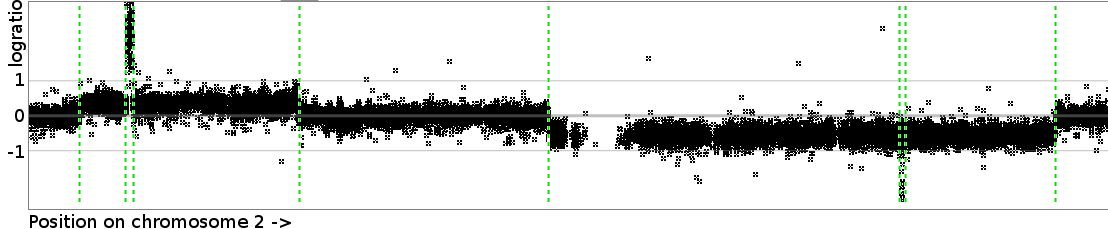
\includegraphics[width=\textwidth]{unlabeled-breakpoints-8}

  Parameter $\lambda_1$ = 8 breakpoints.

  \vskip 0.1in

  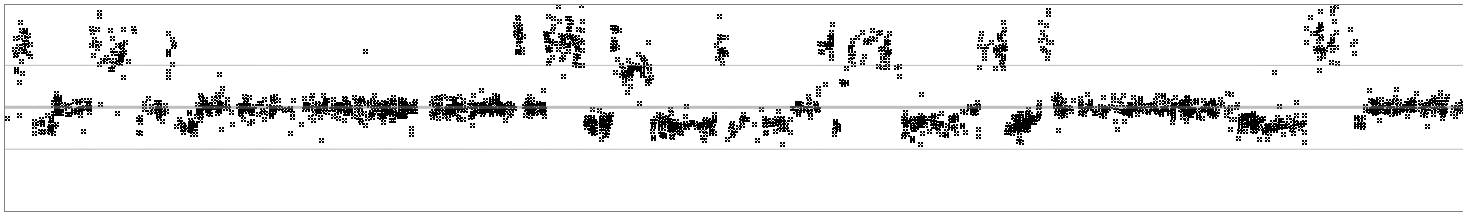
\includegraphics[width=\textwidth]{lots-of-breaks}

  Parameter $\lambda_2$ = ??

  \vskip 0.1in

  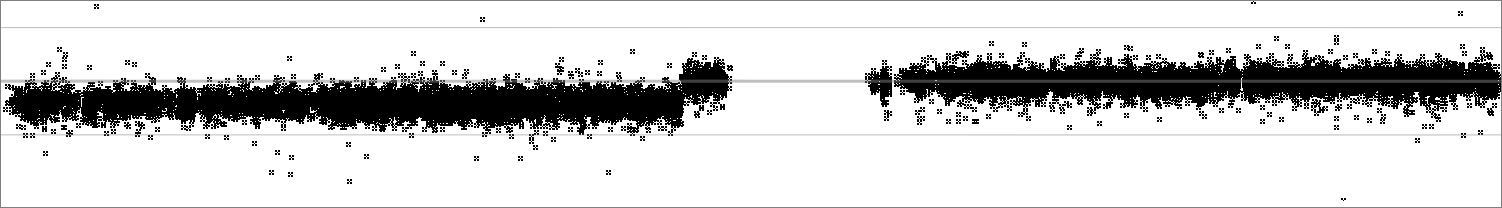
\includegraphics[width=\textwidth]{only-one-break}

  Parameter $\lambda_3$ = ??

\end{frame}

\begin{frame}
  \frametitle{Some problems with unsupervised analysis}
  \textbf{Training a model that works on many samples and genomic
    regions?} 
  \begin{itemize}
  \item What if we don't have time to look at all samples/regions and
      interactively select a good parameter $\lambda$ for each?
  % \item \textbf{Generalization:} how does the parameter for one
  %   profile $\lambda_1$ help us choose a parameter $\lambda_2, \lambda_3$
  %   for other profiles?
  % \item \textbf{What if we use a different model $g(\mathbf x, \rho)$ where
  %   the learned $\lambda$ is meaningless?
  \item Use default parameter $\lambda$ for all profiles?
  \item If we know a good parameter $\lambda_1=8$ for one profile, how
    does that help us choose a parameter $\lambda_2, \lambda_3$ for
    other profiles?
  \end{itemize}
  \textbf{Testing different models of the same data?} 
    \begin{itemize}
    \item   Are the breakpoints of $f(\mathbf x, \lambda$) or
  $g(\mathbf x, \rho)$ better?
    \item Plot the data and both models, qualitative visual evaluation?
    \end{itemize}
  All of these problems can be solved by supervised learning.
\end{frame}

\section{Supervised DNA copy number analysis}

\begin{frame}
  \frametitle{Computer vision: look and add labels to...}
  \begin{tabular}{ccc}
    Photos & Cell images & Copy number profiles \\
    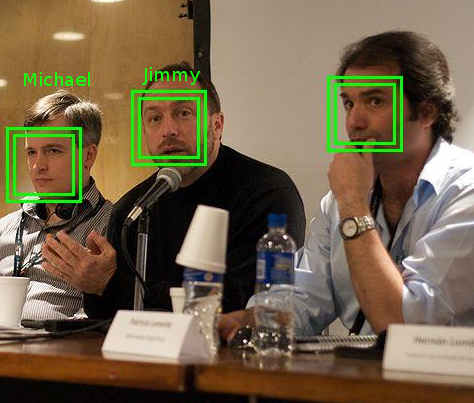
\includegraphics[width=1.3in]{faces} &
    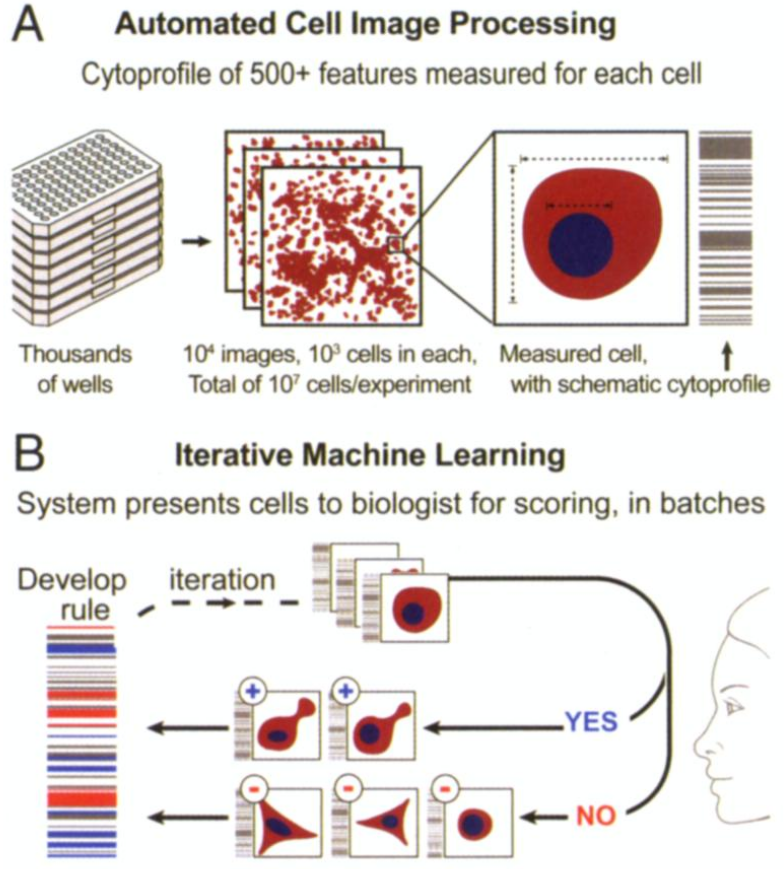
\includegraphics[width=1.3in]{cellprofiler} &
    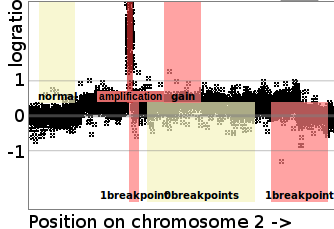
\includegraphics[width=1.5in]{regions-axes}\\
    Labels: faces, names & phenotypes & alterations \\
    CVPR 2013 & CellProfiler & SegAnnDB \\
    246 papers & 873 citations & H, \textit{et al.} 2014. \\
     &
  \end{tabular}
  Sources: \url{http://en.wikipedia.org/wiki/Face_detection}\\
  Jones et al PNAS 2009. Scoring diverse cellular morphologies in
  image-based screens with iterative feedback and machine learning.
\end{frame}

\begin{frame}
  \frametitle{Computer vision for genomic segmentation}
  \begin{center}
  \begin{tabular}{rll}
    \textbf{Breakpoint}\\
 \textbf{detector} & \textbf{strong point} & \textbf{weak point} \\
    \hline
    mathematical  & maximum likelihood & tuning parameters \\
    models & algorithm finds exact  & chosen using\\
& breakpoint locations  & unrealistic assumptions\\
    \hline
    your eyes & outliers, signal/noise & finding the \\
    & over large regions &  exact breakpoint
  \end{tabular}
  \end{center}
  % \vskip 1cm
  % \textbf{SegAnnDB exploits the strong points of both:}
  % \begin{itemize}
  % \item Plot a maximum likelihood model alongside the data.
  % \item Edit annotated regions.
  % \item The model parameters are automatically updated to agree.
  % \item No tuning parameters, but need to annotate a few profiles.
  % \end{itemize}
  % Demo on \url{http://bioviz.rocq.inria.fr/}

  Discussion of common objections:
  \begin{itemize}
  \item \textbf{Isn't this totally subjective?} Yes, guilty as
    charged. \\
    But so is everything else we do, including choice of
    model $f$ and parameter $\lambda$.
  \item \textbf{Won't the results change based on the annotator?}
    Possibly, but usually annotators agree.
  \end{itemize}
\end{frame}



\begin{frame}
  \frametitle{Supervised, non-interactive DNA copy number analysis}

  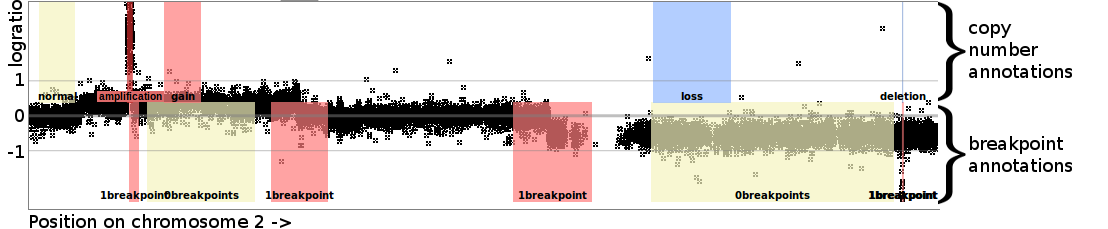
\includegraphics[width=\textwidth]{regions-axes-full}

  Analyst sees a vector of $d$ noisy data points $\mathbf x\in\RR^d$,\\
  and some manually annotated region labels $\mathbf y$.

  \vskip 0.1in

  \sout{\textbf{Question:}\\
    where are the true changes in copy number? (breakpoints)}
  \\
  ``All models are wrong, but some are useful.'' page 424, \textit{Empirical
    Model-Building and Response Surfaces}, Box and Draper (1987).

  \vskip 0.1in

  \textbf{Train question:} can we fit a model $f(\mathbf x, \lambda)$
  to the labels $\mathbf y?$
  \\
  \textbf{Test question:} does the fitted model $f(\mathbf x^*, \lambda)$
  have good predictions for test data $\mathbf x^*$ and labels $\mathbf y^*$?
\end{frame}

\begin{frame}
  \frametitle{Supervised training of breakpoint detection model}

  Reference: Hocking \textit{et al.} Learning smoothing models of copy
  number profiles using breakpoint annotations, BMC Bioinfo
  (2013).

  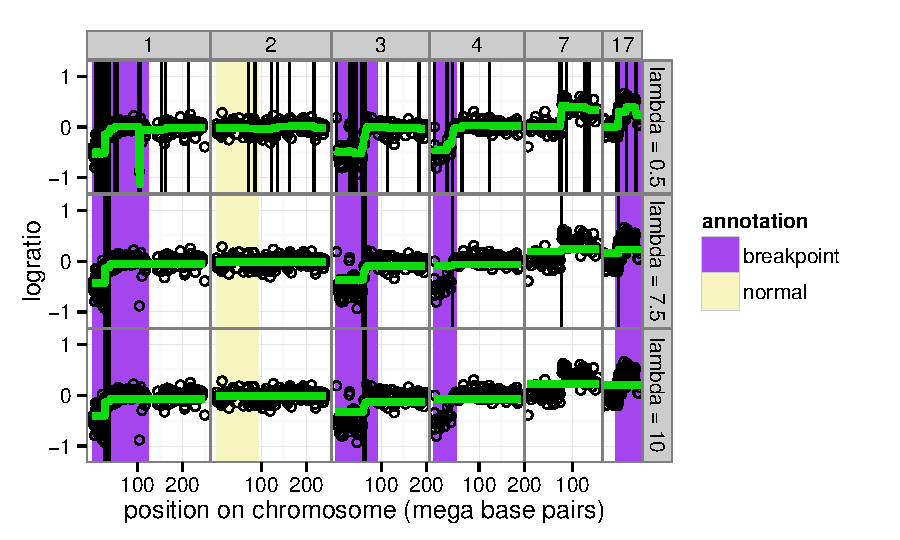
\includegraphics[width=0.8\textwidth]{bams-smoothing}

  \begin{equation*}
    \hat \lambda = \argmin_{\lambda}
    \sum_{i=1}^n
    E\left[
      \mathbf y_i,
      f(\mathbf x_i, \lambda)
    \right]
  \end{equation*}

\end{frame}

\begin{frame}
  \frametitle{Supervised, non-interactive DNA copy number analysis}
  \begin{displaymath}
  \xymatrix{
    \text{Data $\mathbf x$}
    \ar `[r] [dr] 
    \ar [d]
    & \text{ }
    \\
    \text{Plot} 
    \ar [d]
    & 
    \text{Model $f(\mathbf x, \lambda)$} 
    \\
    \text{Labels $\mathbf y$}       
    \ar [d]
    \\
    \text{Parameter $\lambda$} 
    \ar `r[ruu] [ruu]
    & \text{ }
  }
  \end{displaymath}
\end{frame}

\begin{frame}
  \frametitle{Supervised, non-interactive DNA copy number analysis}
  \begin{displaymath}
  \xymatrix{
    \text{Data $\mathbf x$}
    \ar `[r] [dr] 
    \ar [d]
    & \text{ }
    \\
    \text{Plot} 
    \ar [d]
    & 
    \text{Model $f(\mathbf x, \lambda)$} 
    \\
    \text{Labels $\mathbf y$}       
    \ar [d]
    \\
    \text{Parameter $\lambda$} 
    \ar `r[ruu] [ruu]
    & \text{ }
  }
  \end{displaymath}
\end{frame}

\begin{frame}
  \frametitle{Supervised, interactive copy number analysis (SegAnnDB)}

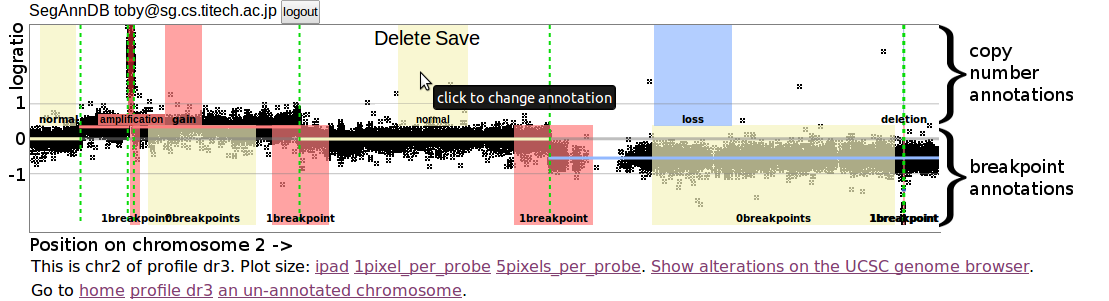
\includegraphics[width=\textwidth]{new-new-annotations}

\vskip 0.2in
Public SegAnnDB server: \url{http://bioviz.rocq.inria.fr/}

\vskip 0.1in
Private server for McGill data sets:
\small
\url{http://ec2-54-201-171-12.us-west-2.compute.amazonaws.com/}

\end{frame}

\begin{frame}
  \frametitle{Supervised, interactive genomic segmentation}
  \small
  \begin{displaymath}
  \xymatrix{
    \text{Data $\mathbf x$}
    \ar `[r] [dr] 
    %\ar `r[rr] [drr] 
    %\ar `r[rrr] [drrr] 
    \ar [d]
    & \text{ }
    & \text{ }
    & \text{ }
    \\
    \text{Plot 1} 
    \ar [d]
    & 
    \text{Model $f(\mathbf x, \lambda_1)$} 
    %\ar [r]
    &
    \color{white}{\text{Plot 2} }
    %\ar [d]
    & 
    \color{white}{\text{Model $f(\mathbf x, \lambda_2)$} }
    \\
    \text{Labels $\mathbf y_1$}       
    \ar [d]
    %\ar [rr]
    %\ar [rru]
    &
    &
    \color{white}{\text{Labels $\mathbf y_2$}}
    %\ar [d]
    \\
    \text{Parameter $\lambda_1$} 
    \ar `r[ruu] [ruu]
    & \text{ }
    & 
    \color{white}{\text{Parameter $\lambda_2$}}
    %\ar `r[ruu] [ruu]
  }
  \end{displaymath}
\end{frame}

\begin{frame}
  \frametitle{Supervised, interactive genomic segmentation}
  \small
  \begin{displaymath}
  \xymatrix{
    \text{Data $\mathbf x$}
    \ar `[r] [dr] 
    \ar `r[rr] [drr] 
    %\ar `r[rrr] [drrr] 
    \ar [d]
    & \text{ }
    & \text{ }
    & \text{ }
    \\
    \text{Plot 1} 
    \ar [d]
    & 
    \text{Model $f(\mathbf x, \lambda_1)$} 
    \ar [r]
    &
    \text{Plot 2} 
    %\ar [d]
    & 
    \color{white}{\text{Model $f(\mathbf x, \lambda_2)$} }
    \\
    \text{Labels $\mathbf y_1$}       
    \ar [d]
    %\ar [rr]
    \ar [rru]
    &
    &
    \color{white}{\text{Labels $\mathbf y_2$}}
    %\ar [d]
    \\
    \text{Parameter $\lambda_1$} 
    \ar `r[ruu] [ruu]
    & \text{ }
    & 
    \color{white}{\text{Parameter $\lambda_2$}}
    %\ar `r[ruu] [ruu]
  }
  \end{displaymath}
\end{frame}

\begin{frame}
  \frametitle{Supervised, interactive genomic segmentation}
  \small
  \begin{displaymath}
  \xymatrix{
    \text{Data $\mathbf x$}
    \ar `[r] [dr] 
    \ar `r[rr] [drr] 
    %\ar `r[rrr] [drrr] 
    \ar [d]
    & \text{ }
    & \text{ }
    & \text{ }
    \\
    \text{Plot 1} 
    \ar [d]
    & 
    \text{Model $f(\mathbf x, \lambda_1)$} 
    \ar [r]
    &
    \text{Plot 2} 
    \ar [d]
    & 
    \color{white}{\text{Model $f(\mathbf x, \lambda_2)$} }
    \\
    \text{Labels $\mathbf y_1$}       
    \ar [d]
    \ar [rr]
    \ar [rru]
    &
    &
    \text{Labels $\mathbf y_2$}
    %\ar [d]
    \\
    \text{Parameter $\lambda_1$} 
    \ar `r[ruu] [ruu]
    & \text{ }
    & 
    \color{white}{\text{Parameter $\lambda_2$}}
    %\ar `r[ruu] [ruu]
  }
  \end{displaymath}
\end{frame}

\begin{frame}
  \frametitle{Supervised, interactive genomic segmentation}
  \small
  \begin{displaymath}
  \xymatrix{
    \text{Data $\mathbf x$}
    \ar `[r] [dr] 
    \ar `r[rr] [drr] 
    %\ar `r[rrr] [drrr] 
    \ar [d]
    & \text{ }
    & \text{ }
    & \text{ }
    \\
    \text{Plot 1} 
    \ar [d]
    & 
    \text{Model $f(\mathbf x, \lambda_1)$} 
    \ar [r]
    &
    \text{Plot 2} 
    \ar [d]
    & 
    \color{white}{\text{Model $f(\mathbf x, \lambda_2)$} }
    \\
    \text{Labels $\mathbf y_1$}       
    \ar [d]
    \ar [rr]
    \ar [rru]
    &
    &
    \text{Labels $\mathbf y_2$}
    \ar [d]
    \\
    \text{Parameter $\lambda_1$} 
    \ar `r[ruu] [ruu]
    & \text{ }
    & \text{Parameter $\lambda_2$}
    %\ar `r[ruu] [ruu]
  }
  \end{displaymath}
\end{frame}


\begin{frame}
  \frametitle{Supervised, interactive genomic segmentation}
  \small
  \begin{displaymath}
  \xymatrix{
    \text{Data $\mathbf x$}
    \ar `[r] [dr] 
    \ar `r[rr] [drr] 
    \ar `r[rrr] [drrr] 
    \ar [d]
    & \text{ }
    & \text{ }
    & \text{ }
    \\
    \text{Plot 1} 
    \ar [d]
    & 
    \text{Model $f(\mathbf x, \lambda_1)$} 
    \ar [r]
    &
    \text{Plot 2} 
    \ar [d]
    & 
    \text{Model $f(\mathbf x, \lambda_2)$} 
    \\
    \text{Labels $\mathbf y_1$}       
    \ar [d]
    \ar [rr]
    \ar [rru]
    &
    &
    \text{Labels $\mathbf y_2$}
    \ar [d]
    \\
    \text{Parameter $\lambda_1$} 
    \ar `r[ruu] [ruu]
    & \text{ }
    & \text{Parameter $\lambda_2$}
    \ar `r[ruu] [ruu]
  }
  \end{displaymath}
\end{frame}

\begin{frame}
  \frametitle{Annotated regions allow supervised and interactive models}
  \begin{tabular}{c|c|c|c}
    Evaluation: & qualitative & quantitative \\
    Input: data + & parameters & annotated regions & Plot/update?\\
    \hline
    & \textbf{unsupervised} & \textbf{supervised} & no\\
    & default & params chosen to \\
    & params & agree w/regions\\
    \hline
    & \textbf{tweaked} & \textbf{interactive} & yes\\
    & params & edit regions
  \end{tabular}
  \begin{description}
  \item[2004-now] dozens of \textbf{unsupervised} models that can be
    \textbf{tweaked} e.g. GLAD, DNAcopy, fused lasso, cghseg, PELT.
  \item[2009-2010] Janoueix-Lerosey, Schleiermacher, et al. J Clinical
    Oncology. Breakpoint region labels recorded by typing 0/1 in Excel
    spreadsheets.
  \item[2013] Hocking et al. BMC Bioinformatics protocols for training
    \textbf{supervised} models.
  \alert<2>{Visual annotations indicate that maximum likelihood
    segmentation is the best (Hocking \textit{et al.}, BMC
    Bioinformatics 2013).}
  \item[2014?] paper about SegAnnDB software for \textbf{interactive}
    genomic segmentation under review, Bioinformatics.
  \end{description}
\end{frame}

\section{Supervised ChIP-seq peak detection}

\begin{frame}
  \frametitle{A brief history of supervised ChIP-seq peak detection}
  \begin{description}
  \item[2011] Rye et al. Manually labeled sites and visual peaks for 3
    transcription factors.\\
    \textbf{Model evaluation.}
  \item[2014] Hocking et al. arXiv:1409.6209. Manually labeled visual
    peaks for 2 histone marks, 4 different annotators.
    \\
    \textbf{Single-parameter model training and evaluation.}\\
    Hocking et al. PeakSeg. NIPS Computational Biology workshop.\\
    \textbf{fo}
  \item[2015] 
  \end{description}
\end{frame}

\begin{frame}
  \frametitle{Two annotators agree on the same profile}
  
  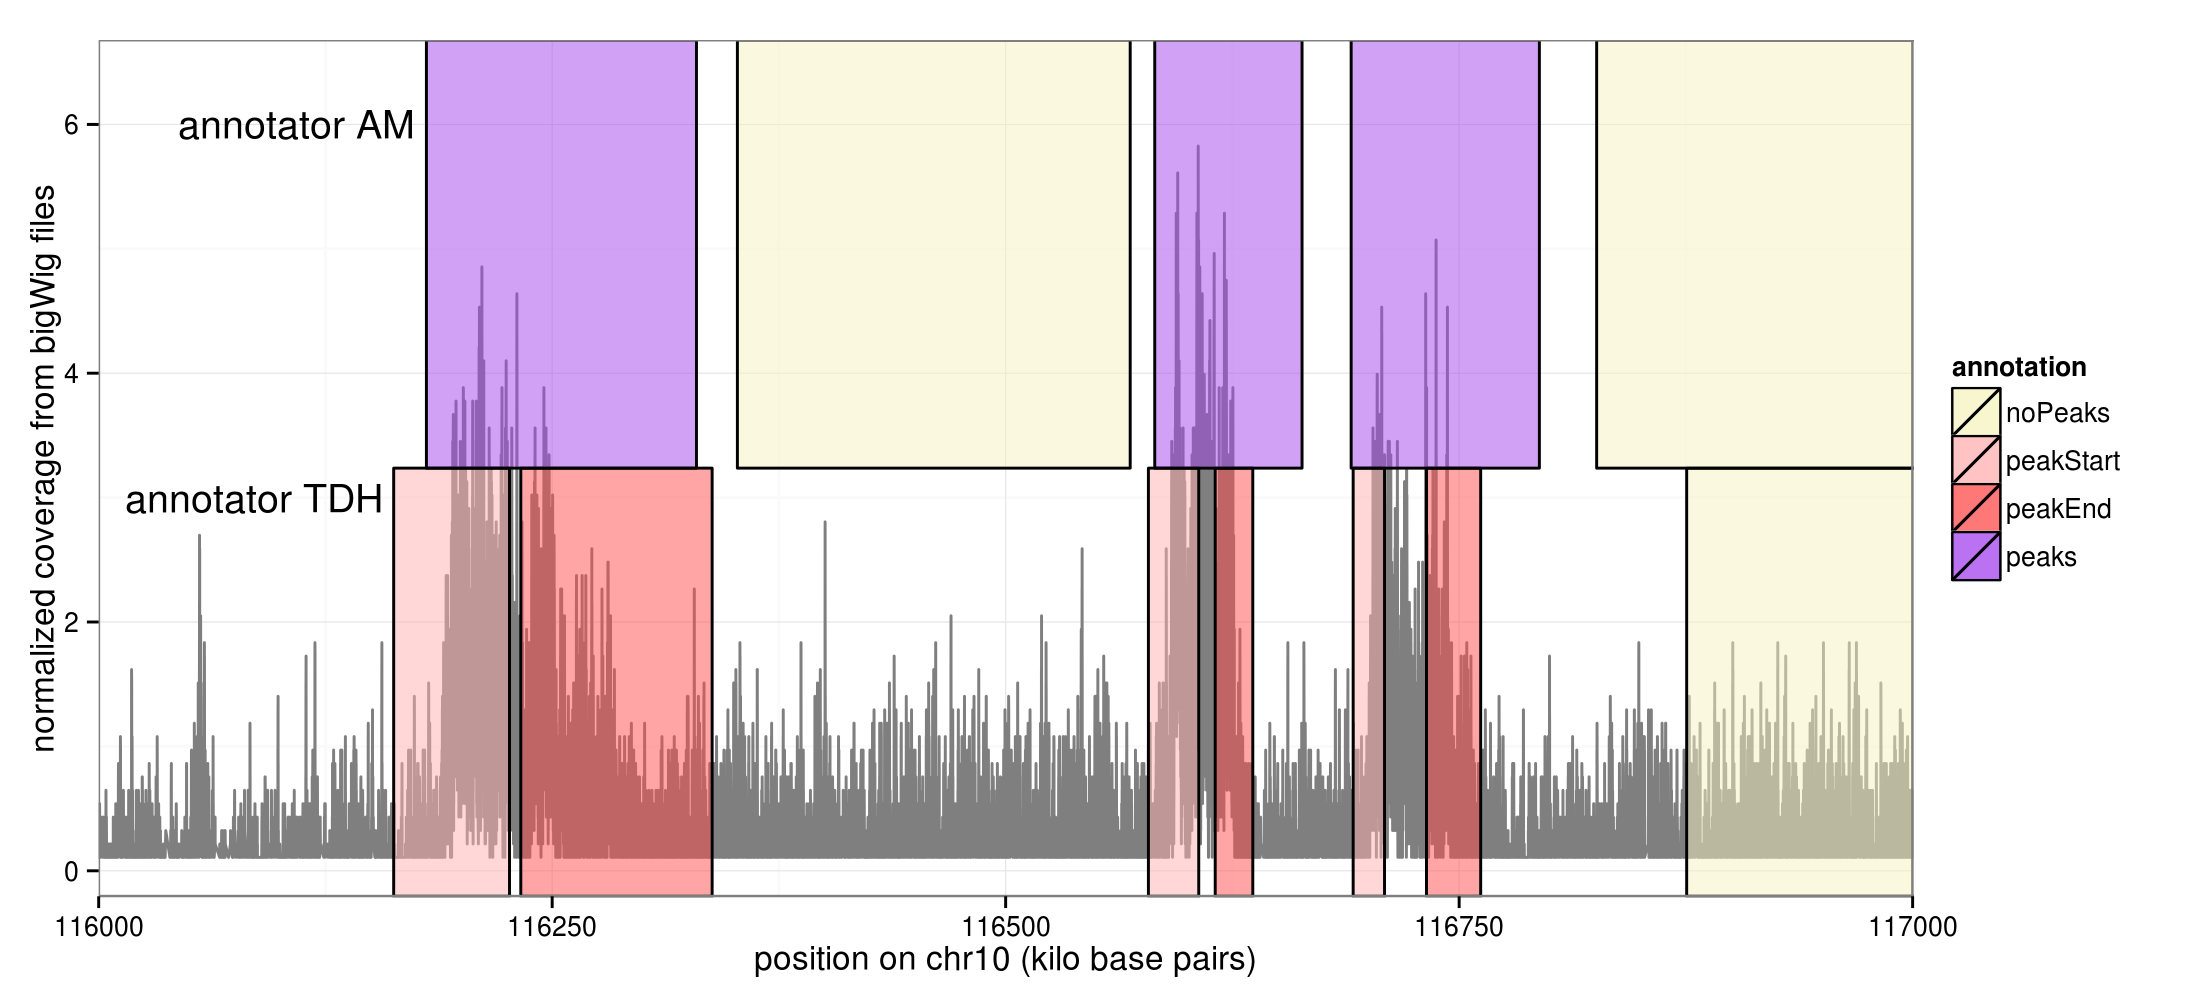
\includegraphics[width=\textwidth]{figure-several-annotators}
\end{frame}

\begin{frame} 
  \frametitle{Advantages of supervised learning}
  Creating data sets $\mathbf x$ with labels $\mathbf y$ is important for
  \begin{description}
  \item[short-term] quantitative evaluation, more convincing papers.
  \item[long-term] cross-discipline collaboration!
    \begin{description}
    \item[statisticians/modelers] get better evaluation
    metrics.
    \item[biologists/annotators] get
    better models.
    \end{description}
  \end{description}

  Can we make labels/supervised approaches for...
  \begin{description}
  \item[segmentation] breakpoint/copy number regions (this work).
  \item[clustering] pairs that should join (or not)?
  \item[regression] variables/genes that are important (or not)?
  \item[diff expression] genes that are up/down (or not)?
  \end{description}
  Write me at \texttt{toby.hocking@mail.mcgill.ca} to collaborate!
\end{frame}

\begin{frame}
  \frametitle{Thank you!}
  Supplementary slides appear after this one.

  \vskip 1cm

  Source code for slides online!\\
  \small
  \url{https://github.com/tdhock/supervised-interactive-slides}
\end{frame}

\end{document}
